\documentclass{llncs}
\usepackage[utf8]{inputenc}
\usepackage{verbatim}
\usepackage{multicol}
\usepackage{llncsdoc}
\usepackage{amsmath}
\usepackage{amsfonts}
\usepackage{amssymb}
\usepackage{graphicx}
\usepackage{lmodern}
\usepackage{calc}
\usepackage{enumitem}
\usepackage{algpseudocode}
\usepackage{algorithm}
\usepackage{algorithmicx}

\algsetblockdefx[IfContinue]{IfContinue}{IfContinue}
{0}{0pt}
[0]{}
[1]{\textbf{if} #1 \textbf{continue}}

\algrenewcommand\algorithmicrequire{%
  \makebox[\widthof{\textbf{Output:}}][l]{\textbf{Input:}}}
  
 \algrenewcommand\algorithmicensure{%
  \textbf{Output:}}

\usepackage{color}
\usepackage{gnuplottex}
\usepackage{subcaption}
\usepackage{microtype}
\usepackage[normalem]{ulem}
\captionsetup{compatibility=false}
\usepackage{tikz}
\usetikzlibrary{trees,automata,positioning}
\usepackage{booktabs}
\usepackage{gnuplottex}
\usepackage{xparse}
\usepackage{epstopdf}
% For scaling gnuplottex
\ExplSyntaxOn
\DeclareExpandableDocumentCommand{\convertlen}{ O{cm} m }
 {
  \dim_to_unit:nn { #2 } { 1 #1 } cm
 }
\ExplSyntaxOff

%% For lattice figure
% Set the overall layout of the tree
\tikzstyle{level 1}=[level distance=3.0cm, sibling distance=0.6cm]
\tikzstyle{level 2}=[level distance=3.5cm, sibling distance=0.6cm]
\tikzstyle{level 3}=[level distance=3.5cm, sibling distance=0.6cm]

% Define styles for bags and leafs
\tikzstyle{l1} = [rectangle, text width=5em, text centered]
\tikzstyle{l2} = [rectangle, text width=5em, text centered]
\tikzstyle{l3} = [rectangle, text width=5em, text centered]

% only when using asmthm
%\newtheorem{definition}{Definition}
%\newtheorem{theorem}{Theorem}

\author{Micky Faas \and Matthijs van Leeuwen}
\title{VOUW: Geometric Pattern Mining using the MDL Principle}
\institute{Leiden Institute for Advances Computer Science}
\begin{document}

\section{Experiments and Results}

To asses the practical performance of the Vouw algorithm, we will primarily use the synthetic dataset generator Ril that was developed specifically for this purpose. Ril utilizes random walks to populate a matrix with patterns of a given size and prevalence, up to a specified density, while filling the remainder of the matrix with noise. Both the pattern elements and the noise are picked from the same uniform random distribution on the interval $[0;255]$. The \emph{signal-to-noise ratio} (SNR) of the data is defined as the number of pattern elements over the matrix size $MN$. The objective of the resulting experiment is that we try to find all of the signal (the patterns) and none of the noise. Figure \ref{fig:ril} gives an overview of what the generated data looks like, how it is mined and evaluated.

\smallskip \noindent \textbf{Implementation.} %
The implementation\footnote{https://github.com/mickymuis/libvouw} that was developed alongside this paper consists of the Vouw algorithm written in vanilla C/C++, a GUI and the synthetic benchmark Ril. All experiments were performed on one core of an Intel Xeon-E2630v3 machine with 512GB RAM.

\smallskip \noindent \textbf{Evaluation.} %
Completely random data (noise) is unlikely to be compressed. The SNR tells us how much noise is present in the data and thus conveniently gives us an upper bound of how much compression could be achieved. We use the ground truth SNR versus the resulting compression ratio as a benchmark to tell us how close we are in finding all the structure in the ground truth. 

Because the compression ratio alone does not tell us the quality of the results, we also compare the ground truth matrix with the compressed result. In order to do this, we use the notion that elements that have been encoded with singleton patterns, could evidently not be compressed. These elements must therefore be noise. We reconstruct the original matrix from the compressed result, while we omit any singleton patterns. This essentially gives us a matrix of `positives' (signal) and `negatives' (noise). By comparing each element with the corresponding element in the ground truth matrix, the \emph{true positives} can be calculated. This subsequently gives us traditional figures for \emph{precision} and \emph{recall}.

Figure \ref{fig:snr} plots input SNR versus compression as well as precision/recall for different matrix sizes. We expect the resulting compression ratio to be close to $1-\mathrm{snr}$. In Figure \ref{fig:usage} shows that patterns with a low prevalence have a lower probability of being `detected' by the algorithm as they are more likely to by accidental/noise. We see that increasing the matrix size also increases this threshold. Finally we look at the influence of the two improvements upon the baseline algorithm as described in Section \ref{improvements}. Table \ref{table:optimize} shows both precision/recall figures as well as wall clock time. In terms of quality, local search improves the results quite substantial in some cases (other experiments have shown that it can dramatically lower the detection threshold as well) while Best-N notably lowers precision. Both improve speed by an order of magnitude, although the improvements given by Best-N are clearly superior. %Another observation is that the baseline algorithm does not scale very favourable with matrix size and that these improvements may be a requisite when mining larger matrices.    


%%
%% The following LaTeX + Gnuplot code generates the two graphs using the gnuplottex package
%% It can be omitted by directly including the pre-baked PDFs as figures
%%
\begin{comment}

\begin{figure}[p]%
	%\centering%
	\begin{subfigure}[t]{0.5\textwidth}
	%\centering
	\begin{gnuplot}[terminal=epslatex, terminaloptions={color dashed size 6.5cm,6cm font "lmodern,8"}]
		set key box bottom left
		set key width 1.0
		set key height 1.0
		set key spacing 1.1
		set key opaque
		set sample 1000
		set xr [0:.7]
		set yr [0:1]
		set grid xtics lt 0 ls 0
		set grid ytics lt 0 ls 0
		set xlabel 'Signal-to-noise Ratio'
		set ylabel 'Compression'
		#plot "data/256_snr_vs_prec_n10.txt" w l lc 1 lw 1 t "precision",\
		#	 "data/256_snr_vs_recall_n10.txt" w l lc 2 lw 1 t "recall",\
		#	 "data/256_snr_vs_compr_n10.txt" w l lc 3 lw 1 t "ratio"
		plot "data/output_snr_256.txt" using 4:5 w l lc 1 lw 2.5 t "256",\
  			 "data/output_snr_512.txt" using 4:5 w l lc 2 lw 2.5 t "512",\
  			 "data/output_snr_1024.txt" using 4:5 w l lc 3 lw 2.5 t "1024",\
  			 "data/output_snr_2048.txt" using 4:5 w l lc 4 lw 2.5 t "2048"
	\end{gnuplot}}\
	\caption{The influence of SNR in the ground truth}
	\label{fig:snr}
	\end{subfigure}%
	%\vspace{-\baselineskip}
	~
	\begin{subfigure}[t]{0.5\textwidth}
	%\centering
	\begin{gnuplot}[terminal=epslatex, terminaloptions={color dashed size 6.5cm,6cm font "lmodern,8"}]
		set key box bottom right
		set key width 1.0
		set key height 1.0
		set key spacing 1.1
		set key opaque
		set sample 1000
		set xr [0:50]
		set yr [0:1]
		set grid xtics lt 0 ls 0
		set grid ytics lt 0 ls 0
		set xlabel 'Prevalence per Pattern'
		set ylabel 'Recall' offset 1,0,0
		plot "data/usage_test_128.txt" using 1:8 w l lc 1 lw 2.5 t "128",\
			 "data/usage_test_256.txt" using 1:8 w l lc 2 lw 2.5 t "256",\
			 "data/usage_test_512.txt" using 1:8 w l lc 3 lw 2.5 t "512",\
			 "data/usage_test_1024.txt" using 1:8 w l lc 4 lw 2.5 t "1024"
	\end{gnuplot}
	%\vspace{-\baselineskip}
	\caption{Prevalence versus recall}
	\label{fig:usage}
	\end{subfigure}
	\caption{}
	\label{fig:plots}
\end{figure}
\end{comment}

%%
%% End of Gnuplottex section
%%

% Begin of proxy graphs from PDF

\begin{figure}[p]%
	\begin{subfigure}[t]{0.5\textwidth}
	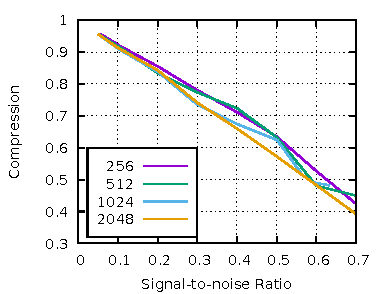
\includegraphics[scale=1]{figures/experiments-gnuplottex-fig1.pdf}
	\caption{The influence of SNR in the ground truth}
	\label{fig:snr}

	\end{subfigure}%
	%\vspace{-\baselineskip}
	~
	\begin{subfigure}[t]{0.5\textwidth}
	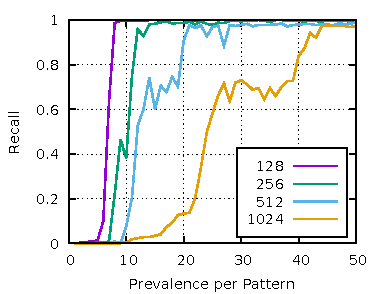
\includegraphics[scale=1]{figures/experiments-gnuplottex-fig2.pdf}
	%\vspace{-\baselineskip}
	\caption{Prevalence versus recall}
	\label{fig:usage}
	\end{subfigure}
	\caption{}
	\label{fig:plots}
\end{figure}

% End of proxy graphs

\begin{figure}[p]
\centering
\begin{subfigure}[t]{0.25\textwidth}
\centering
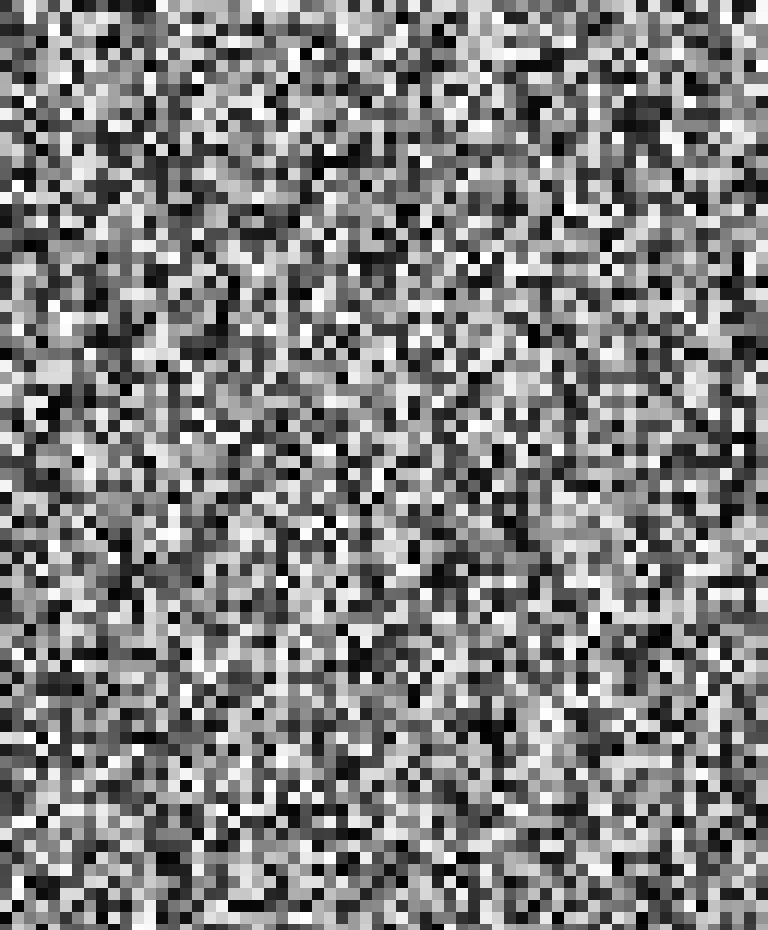
\includegraphics[scale=.9]{img/exp_input_2_cropped.png}
\caption{Generated matrix}
\label{fig:rila}
\end{subfigure}%
~
\begin{subfigure}[t]{0.25\textwidth}
\centering
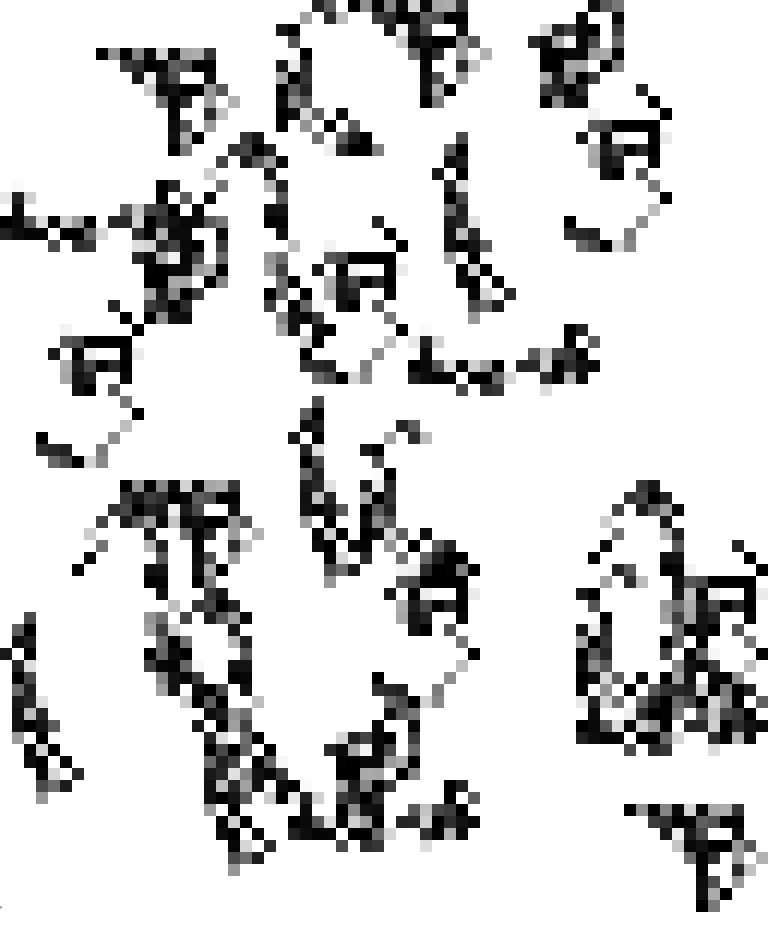
\includegraphics[scale=.9]{img/exp_inputpatterns_2_cropped.png}
\caption{Ground truth patterns}
\label{fig:rilb}
\end{subfigure}%
~
\begin{subfigure}[t]{0.25\textwidth}
\centering
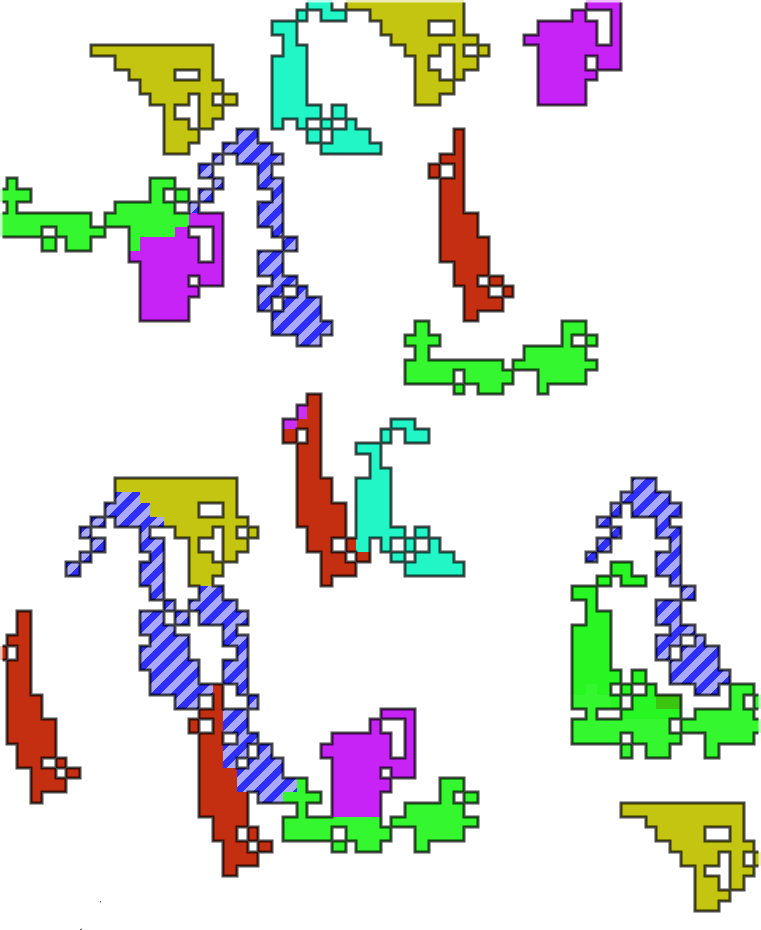
\includegraphics[scale=.9]{img/exp_result_2_cropped.png}
\caption{Found patterns}
\label{fig:rilc}
\end{subfigure}%
~
\begin{subfigure}[t]{0.25\textwidth}
\centering
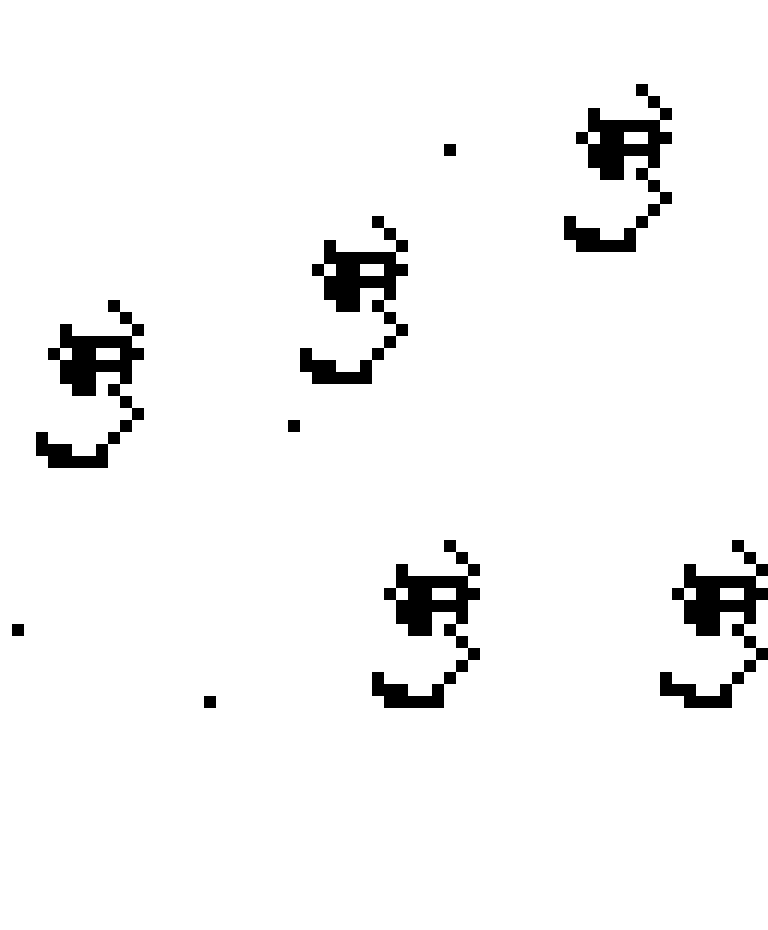
\includegraphics[scale=.9]{img/exp_diff_2_cropped.png}
\caption{Difference}
\label{fig:rild}
\end{subfigure}%
\caption{Example of how synthetic input is generated and evaluated.}
\label{fig:ril}
\end{figure}  

\begin{table}[p]
%\centering
\caption{Influence of optimizations with respect to the baseline algorithm}
\label{table:optimize}
\begin{tabular*}{\textwidth}{c @{\extracolsep{\fill}}llcccccccc}
\toprule
 & & \multicolumn{4}{c}{Precision/Recall} & \multicolumn{4}{c}{Average time}\\
 \cmidrule(r){3-6} \cmidrule(r){7-10} 
 Size & SNR & None & Local & Best-N & Both & None & Local & Best-N & Both \\
\midrule
 256 & .05 & .98/.98 & .99/.99 & .93/.98 & .95/.99 & 29s & 1s & 2s & 1s \\
   & .3 &.99/.8 & .99/.88 & .96/.82 & .99/.89 & 2m 32s & 9s & 5s & 5s \\
 512 & .05 & .98/.97 & .99/.99 & .87/.97 & .93/.98 & 5m 26s & 8s & 20s & 6s \\
  & .3 &.97/.93 & .99/.99 & .94/.91 & .97/.90 & 26m 52s & 2m 32s & 24s & 65s \\
 1024 & .05 & .97/.98 & .99/.99 & .84/.98 & .92/.96 & 21m 34s & 44s & 37s & 34s \\
 & .3 &.98/.98 & .99/.99 & .93/.96 & .98/.97 & 116m & 7m 31s & 1m 49s & 3m 31s \\
\bottomrule
\end{tabular*}
%\caption*{$^1$ signal-to-noise ratio of $.05$, $^2$ signal-to-noise ratio of $.3$}
\end{table}

\end{document}
